%!TEX root = ../main.tex
\section{Cognitive Architecture and LLMs Integration}\label{background}
\subsection{Production Systems}
In symbolic AI, when it comes to \emph{production
systems}~\cite{humanproblemsolving} we refer to the reduction of mathematics and
computation to \emph{symbolic manipulation} and more in general, production
systems have been proposed as a formalism to think about arbitrary logical
systems~\cite{Post1943-POSFRO} which later will be shown to be equivalent to a
simpler string rewriting system. Thanks to this approach, complex behaviours
could emerge from quite simple production systems. The large adoption by the AI
community of production systems came from their generalisation to
\textbf{logical operations}: \emph{preconditions} that could be checked against
agent's \emph{goals} and \emph{world} state, and \emph{actions} that should be
taken if preconditions are satisfied.

\subsection{Cognitive Architectures}
The usage of large production systems connected to external sensors, actuator
and knowledge bases, required a sophisticated control flow: a \textbf{Cognitive
Architecture}~\cite{LANGLEY2009141}. A typical Soar
Architecture~\cite{Newell1990-NEWUTO} as shown in \Cref{fig:soar}, is composed
by four major concepts:
\begin{itemize}
    \item \textbf{Memory}: multiple memories, mainly divided into \emph{short term working memory} which reflects agent's current circumstances (perceptual inputs, goals, intermediate results), and a \emph{long term memory} which is divided into a
    \begin{enumerate*}[label=(\emph{\roman{*}})]
        \item \emph{procedural memory} containing the production system, a
        \item \emph{semantic memory} which stores facts about the world and the agent itself, and a
        \item \emph{episodic memory} keeping track of agent's past behaviours.
    \end{enumerate*}
    \item \textbf{Grounding}: in embodied context percepts are generated by sensors as agent's inputs, also equipping the Soar agent with actuators allowing physical interactions.
    \item \textbf{Decision Making} accomplished through a decision loop that
    \begin{enumerate*}[label=(\emph{\roman{*}})]
        \item matches preconditions from procedural memory,
        \item checks preconditions against agent's working memory,
        \item through a \emph{propose and evaluate phase} actions ranking and selections is performed for then
        \item choose, produce and execute the action.
    \end{enumerate*}
    \item \textbf{Learning} is supported by the Soar architecture through various forms, where in the most basic ways, facts are written in to semantic memory and experiences in episodic memory. Even behaviours can be modified by rewriting through \ac{RL} or adding new productions to the procedural memory.
\end{itemize}

Cognitive architectures have become less popular over the last few decades
reflecting two main problems: they're \emph{limited to domains} that can be
described with logical predicates, and require many pre-specified rules in order
to function properly.

\begin{figure*}
    \centering
    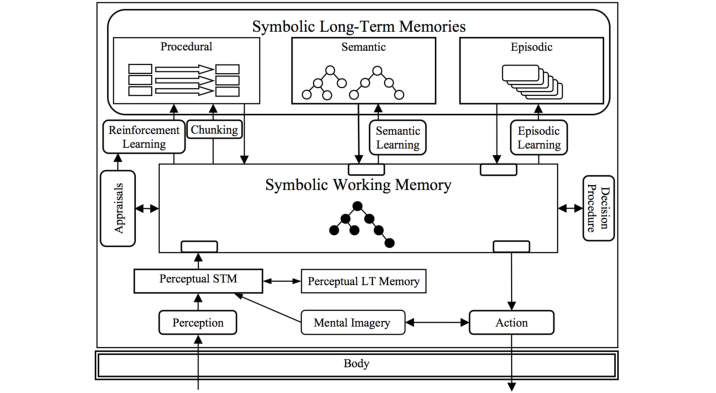
\includegraphics[width=\textwidth]{img/The-Soar-cognitive-architecture.png}
    \caption{The Soar Architecture}
    \label{fig:soar}
\end{figure*}
